\chapter{HASIL}

\section{Pengambilan Data Lokasi}

Data yang digunakan adalah data koordinat lokasi yang diekspor melalui Google Earth. Lokasi pada Google Earth ditandai satu per satu dan diekspor ke dalam bentuk spreadsheet. Dapat dilihat pada Lampiran \ref{lampiran1} seluruh nama-nama SMA di Kabupaten Probolinggo beserta koordinat lokasinya. Data tersebut dikumpulkan sebagai dataset dari penelitian ini. Visualisasi data dari koordinat-koordinat SMA di kabupaten probolinggo dapat dilihat pada Gambar \ref{fig:petasma}.

\begin{figure}[H]
  \centering
  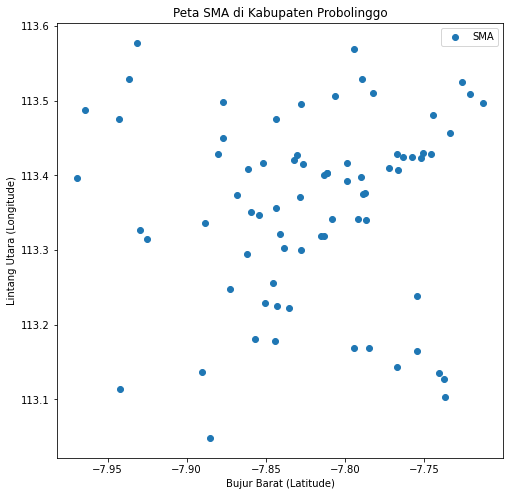
\includegraphics[width=0.5\textwidth]{Gambar/peta sma.png}
  \caption{Visualisasi lokasi SMA di Kabupaten Probolinggo}
  \label{fig:petasma}
\end{figure}

Setelah peneliti mendapatkan lokasi yang akan diproses, selanjutnya diuji menggunakan pembagian dari 1 sampai dengan 10 klaster untuk mengetahui rute dan pembagian klaster yang paling optimal. Berikut ini adalah hasil dari percobaan tersebut.

\section{Proses Pengklasteran Data}

Pada tahap ini metode yang digunakan adalah metode $k-$means untuk mengklaster data. Langkah-langkah nya adalah sebagai berikut.

\begin{enumerate}
	\item Tentukan jumlah klaster, dalam hal ini yang digunakan adalah ujicoba dengan pembagian 1 sampai dengan 10 klaster.
	\item Selanjutnya pilih titik-titik centroid secara acak sebanyak jumlah klaster. Dari hasil pemilihan acak tersebut terpilihlah titik-titik centroid berikut.
	
	\begin{enumerate}
	
	\item Untuk pembagian 1 klaster terpilih titik-titik centroid pada Tabel \ref{tab:center1}.
	
\begin{table}[H]
\footnotesize
\centering
\begin{tabular}{ccc}
\rowcolor[HTML]{4472C4} 
{\color[HTML]{FFFFFF} \textbf{Nama   Centroid}} & {\color[HTML]{FFFFFF} \textbf{Latitude (Sumbu X)}} & {\color[HTML]{FFFFFF} \textbf{Longitude (Sumbu Y)}} \\
\rowcolor[HTML]{D9E1F2} 
A &
  -7,77 &
  113,41
\end{tabular}
\caption{Centroid pada 1 klaster}
\label{tab:center1}
\end{table}


	\item Untuk pembagian 2 klaster terpilih titik-titik centroid pada Tabel \ref{tab:center2}.

\begin{table}[H]
\footnotesize
\centering
\begin{tabular}{ccc}
\rowcolor[HTML]{4472C4} 
{\color[HTML]{FFFFFF} \textbf{Nama   Centroid}} & {\color[HTML]{FFFFFF} \textbf{Latitude (Sumbu X)}} & {\color[HTML]{FFFFFF} \textbf{Longitude (Sumbu Y)}} \\
\rowcolor[HTML]{D9E1F2} 
A                                               & -7,75                                              & 113,42                                              \\
B                                               & -7,83                                              & 113,30                                             
\end{tabular}
\caption{Centroid pada 2 klaster}
\label{tab:center2}
\end{table}

	\item Untuk pembagian 3 klaster terpilih titik-titik centroid pada Tabel \ref{tab:center3}.
	
\begin{table}[H]
\footnotesize
\centering
\begin{tabular}{ccc}
\rowcolor[HTML]{4472C4} 
{\color[HTML]{FFFFFF} \textbf{Nama   Centroid}} & {\color[HTML]{FFFFFF} \textbf{Latitude (Sumbu X)}} & {\color[HTML]{FFFFFF} \textbf{Longitude (Sumbu Y)}} \\
\rowcolor[HTML]{D9E1F2} 
A & -7,84 & 113,22 \\
B & -7,93 & 113,31 \\
\rowcolor[HTML]{D9E1F2} 
C & -7,79 & 113,38
\end{tabular}
\caption{Centroid pada 3 klaster}
\label{tab:center3}
\end{table}

	\item Untuk pembagian 4 klaster terpilih titik-titik centroid pada Tabel \ref{tab:center4}.
	
\begin{table}[H]
\footnotesize
\centering
\begin{tabular}{ccc}
\rowcolor[HTML]{4472C4} 
{\color[HTML]{FFFFFF} \textbf{Nama   Centroid}} & {\color[HTML]{FFFFFF} \textbf{Latitude (Sumbu X)}} & {\color[HTML]{FFFFFF} \textbf{Longitude (Sumbu Y)}} \\
\rowcolor[HTML]{D9E1F2} 
A & -7,77 & 113,43 \\
B & -7,83 & 113,42 \\
\rowcolor[HTML]{D9E1F2} 
C & -7,74 & 113,13 \\
D & -7,75 & 113,42
\end{tabular}
\caption{Centroid pada 4 klaster}
\label{tab:center4}
\end{table}	
	
	\item Untuk pembagian 5 klaster terpilih titik-titik centroid pada Tabel \ref{tab:center5}
	
\begin{table}[H]
\footnotesize
\centering
\begin{tabular}{ccc}
\rowcolor[HTML]{4472C4} 
{\color[HTML]{FFFFFF} \textbf{Nama   Centroid}} & {\color[HTML]{FFFFFF} \textbf{Latitude (Sumbu X)}} & {\color[HTML]{FFFFFF} \textbf{Longitude (Sumbu Y)}} \\
\rowcolor[HTML]{D9E1F2} 
A & -7,94 & 113,11 \\
B & -7,85 & 113,42 \\
\rowcolor[HTML]{D9E1F2} 
C & -7,80 & 113,39 \\
D & -7,94 & 113,53 \\
\rowcolor[HTML]{D9E1F2} 
E & -7,84 & 113,32
\end{tabular}
\caption{Centroid pada 5 klaster}
\label{tab:center5}
\end{table}

	\item Untuk pembagian 6 klaster terpilih titik-titik centroid pada Tabel \ref{tab:center6}.
	
\begin{table}[H]
\footnotesize
\centering
\begin{tabular}{ccc}
\rowcolor[HTML]{4472C4} 
{\color[HTML]{FFFFFF} \textbf{Nama   Centroid}} & {\color[HTML]{FFFFFF} \textbf{Latitude (Sumbu X)}} & {\color[HTML]{FFFFFF} \textbf{Longitude (Sumbu Y)}} \\
\rowcolor[HTML]{D9E1F2} 
A & -7,79 & 113,53 \\
B & -7,86 & 113,29 \\
\rowcolor[HTML]{D9E1F2} 
C & -7,89 & 113,14 \\
D & -7,87 & 113,37 \\
\rowcolor[HTML]{D9E1F2} 
E & -7,94 & 113,48 \\
F & -7,88 & 113,50
\end{tabular}
\caption{Centroid pada 6 klaster}
\label{tab:center6}
\end{table}

	\item Untuk pembagian 7 klaster terpilih titik-titik centroid pada Tabel \ref{tab:center7}.
	
\begin{table}[H]
\footnotesize
\centering
\begin{tabular}{ccc}
\rowcolor[HTML]{4472C4} 
{\color[HTML]{FFFFFF} \textbf{Nama   Centroid}} & {\color[HTML]{FFFFFF} \textbf{Latitude (Sumbu X)}} & {\color[HTML]{FFFFFF} \textbf{Longitude (Sumbu Y)}} \\
\rowcolor[HTML]{D9E1F2} 
A & -7,89 & 113,34 \\
B & -7,81 & 113,32 \\
\rowcolor[HTML]{D9E1F2} 
C & -7,84 & 113,48 \\
D & -7,79 & 113,17 \\
\rowcolor[HTML]{D9E1F2} 
E & -7,71 & 113,50 \\
F & -7,77 & 113,41 \\
\rowcolor[HTML]{D9E1F2} 
G & -7,72 & 113,51
\end{tabular}
\caption{Centroid pada 7 klaster}
\label{tab:center7}
\end{table}

	\item Untuk pembagian 8 klaster terpilih titik-titik centroid pada Tabel \ref{tab:center8}.
	
\begin{table}[H]
\footnotesize
\centering
\begin{tabular}{ccc}
\rowcolor[HTML]{4472C4} 
{\color[HTML]{FFFFFF} \textbf{Nama   Centroid}} & {\color[HTML]{FFFFFF} \textbf{Latitude (Sumbu X)}} & {\color[HTML]{FFFFFF} \textbf{Longitude (Sumbu Y)}} \\
\rowcolor[HTML]{D9E1F2} 
A & -7,79 & 113,38 \\
B & -7,88 & 113,43 \\
\rowcolor[HTML]{D9E1F2} 
C & -7,78 & 113,51 \\
D & -7,84 & 113,30 \\
\rowcolor[HTML]{D9E1F2} 
E & -7,75 & 113,43 \\
F & -7,75 & 113,16 \\
\rowcolor[HTML]{D9E1F2} 
G & -7,86 & 113,18 \\
H & -7,86 & 113,35
\end{tabular}
\caption{Centroid pada 8 klaster}
\label{tab:center8}
\end{table}

	\item Untuk pembagian 9 klaster terpilih titik-titik centroid pada Tabel \ref{tab:center9}.
	
\begin{table}[H]
\footnotesize
\centering
\begin{tabular}{ccc}
\rowcolor[HTML]{4472C4} 
{\color[HTML]{FFFFFF} \textbf{Nama   Centroid}} & {\color[HTML]{FFFFFF} \textbf{Latitude (Sumbu X)}} & {\color[HTML]{FFFFFF} \textbf{Longitude (Sumbu Y)}} \\
\rowcolor[HTML]{D9E1F2} 
A & -7,83 & 113,30 \\
B & -7,74 & 113,48 \\
\rowcolor[HTML]{D9E1F2} 
C & -7,84 & 113,22 \\
D & -7,93 & 113,31 \\
\rowcolor[HTML]{D9E1F2} 
E & -7,79 & 113,38 \\
F & -7,88 & 113,43 \\
\rowcolor[HTML]{D9E1F2} 
G & -7,78 & 113,51 \\
H & -7,84 & 113,30 \\
\rowcolor[HTML]{D9E1F2} 
I & -7,75 & 113,43 \\                        
\end{tabular}
\caption{Centroid pada 9 klaster}
\label{tab:center9}
\end{table}

	\item Untuk pembagian 10 klaster terpilih titik-titik centroid pada Tabel \ref{tab:center10}.
	
\begin{table}[H]
\centering
\footnotesize
\begin{tabular}{ccc}
\rowcolor[HTML]{4472C4} 
{\color[HTML]{FFFFFF} \textbf{Nama   Centroid}} & {\color[HTML]{FFFFFF} \textbf{Latitude (Sumbu X)}} & {\color[HTML]{FFFFFF} \textbf{Longitude (Sumbu Y)}} \\
\rowcolor[HTML]{D9E1F2} 
A & -7,77 & 113,41 \\
B & -7,76 & 113,43 \\
\rowcolor[HTML]{D9E1F2} 
C & -7,84 & 113,18 \\
D & -7,83 & 113,50 \\
\rowcolor[HTML]{D9E1F2} 
E & -7,87 & 113,25 \\
F & -7,94 & 113,11 \\
\rowcolor[HTML]{D9E1F2} 
G & -7,85 & 113,42 \\
H & -7,80 & 113,39 \\
\rowcolor[HTML]{D9E1F2} 
I & -7,94 & 113,53 \\
J & -7,84 & 113,32
\end{tabular}
\caption{Centroid pada 10 klaster}
\label{tab:center10}
\end{table}

		
	\end{enumerate}

	\item \label{ulang3} Hitung jarak tiap titik sekolah yang ada dengan masing-masing \textit{centroid}. Penghitungan jarak menggunakan \textit{Euclidean distance} pada persamaan (\ref{eq:euclidean3}).
	
	\begin{equation}
	\left[ \left( x,y \right) ,\left( a,b \right)\right]=\sqrt{\left( x-a \right)^{2}+\left( y-b \right)^{2}}
	\label{eq:euclidean3}
	\end{equation}	
	
	\item Kelompokan data ke dalam klaster yang memiliki jarak paling minimum.
	\item Setelah seluruh titik sekolah masuk ke dalam klaster-klaster, hitung \textit{centroid} yang baru dengan cara menghitung rata-rata titik sekolah yang ada di dalam klaster tersebut. Lakukan hal yang sama pada klaster yang lain.
	\item Jika terdapat perubahan klaster, maka ulangi langkah \ref{ulang3} hingga tidak ada perubahan anggota pada tiap klaster. Jika \textit{centroid} yang baru tidak berubah dari sebelumnya, maka proses berhenti, karena \textit{centroid} yang tidak berubah menyebabkan anggota klaster juga tidak berubah.
	
	\item Setelah semua data terklasifikasi, selanjutnya adalah menentukan titik kumpul dengan cara menghitung rata-rata dari seluruh titik-titik centroid tersebut.
\end{enumerate}

\section{Proses TSP menggunakan Algoritma Genetika}

Setelah data terklaster seperti pada Gambar \ref{fig:hasilklas} selanjutnya adalah mencari rute terdekatnya menggunakan algoritma genetika

\begin{figure}[H]
	\centering
	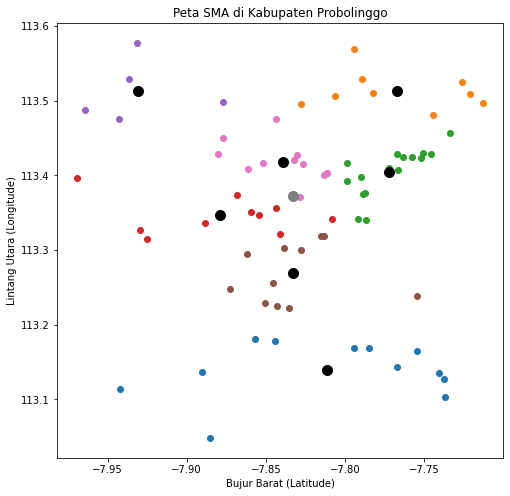
\includegraphics[width=0.5\textwidth]{Gambar/hasil klaster.png}
	\caption{Visualisasi klaster sesuai warna}
	\label{fig:hasilklas}
\end{figure}

\begin{enumerate}
	\item Bangkitkan beberapa populasi awal berisi sejumlah kromosom yang di dalamnya terdapat urutan perjalanan menuju titik sekolah.
	\item \label{ulang4} Hitung nilai \textit{fitness} (total jarak) dari tiap kromosom.
	\item Menetapkan probabilitas \textit{crossover} ($p_c$) dalam hal ini yang digunakan adalah $p_c=0,95$. Bangkitkan bilangan acak (0,0000 sampai 1,0000) pada setiap kromosom, kromosom dengan bilangan acak kurang dari $p_c$ maka akan dilakukan \textit{crossover}. Jika kromosom hasil \textit{crossover} memiliki \textit{fitness} yang lebih baik  dari kromosom awal, maka kromosom awal digantikan oleh kromosom hasil \textit{crossover}.
	\item Menetapkan probabilitas mutasi ($p_m$), dalam hal ini digunakan $p_m=0,1$. Bangkitakan bilangan acak (0,0000 sampai 1,0000) pada setiap kromosom, kromosom yang memiliki bilangan acak kurang dari $p_m$ maka akan dilakukan mutasi. Jika kromosom hasil mutasi memiliki \textit{fitness} yang lebih baik dari kromosom awal, maka kromosom awal digantikan oleh kromosom hasil mutasi.
	\item Jika hasil kurang optimal, iterasi dilakukan dengan cara kembali ke tahapan (\ref{ulang4}) untuk generasi berikutnya sampai hasil yang dilakukan optimal atau mendekati optimal.
\end{enumerate}

\section{Hasil akhir}

Dari serangkaian proses di atas, menghasilkan beberapa rute optimal yang dapat dilalui yang merupakan rute yang didapatkan dari pembagian klaster berbeda. Salah satunya pada Gambar \ref{fig:hasil_mtsp1} tidak menggunakan pembagian klaster, sehingga titik centroid pada klaster tersebut dijadikan titik kumpul.

Rute-rute yang dihasilkan sebelumnya diekspor ke bentuk spreadsheet dan telah diurutkan berdasarkan nomor urut yang terdapat pada Lampiran \ref{lampiran1} sehingga mempermudah pengguna dalam membaca data.

\subsection{Tanpa pembagian klaster}

Urutan perjalanan perjalanan dengan tanpa pembagian klaster menghasilkan urutan titik seperti berikut. $K$-means pada urutan ini tidak digunakan untuk pengklasteran data, namun hanya untuk penentuan titik kumpul.

\noindent $
67 \rightarrow 30 \rightarrow 52 \rightarrow 38 \rightarrow 37 \rightarrow 50 \rightarrow 62 \rightarrow 25 \rightarrow 14 \rightarrow 7 \rightarrow 27 \rightarrow 17 \rightarrow 23 \rightarrow 69 \rightarrow 72 \rightarrow 21 \rightarrow 55 \rightarrow 54 \rightarrow 20 \rightarrow 46 \rightarrow 26 \rightarrow 59 \rightarrow 60 \rightarrow 16 \rightarrow 58 \rightarrow 45 \rightarrow 15 \rightarrow 65 \rightarrow 36 \rightarrow 18 \rightarrow 40 \rightarrow 70 \rightarrow 75 \rightarrow 2 \rightarrow 44 \rightarrow 11 \rightarrow 41 \rightarrow 53 \rightarrow 3 \rightarrow 71 \rightarrow 10 \rightarrow 6 \rightarrow 29 \rightarrow 74 \rightarrow 68 \rightarrow 47 \rightarrow 32 \rightarrow 56 \rightarrow 63 \rightarrow 9 \rightarrow 51 \rightarrow 49 \rightarrow 35 \rightarrow 1 \rightarrow 73 \rightarrow 24 \rightarrow 33 \rightarrow 57 \rightarrow 61 \rightarrow 22 \rightarrow 34 \rightarrow 8 \rightarrow 43 \rightarrow 66 \rightarrow 42 \rightarrow 13 \rightarrow 5 \rightarrow 4 \rightarrow 64 \rightarrow 31 \rightarrow 39 \rightarrow 19 \rightarrow 28 \rightarrow 48 \rightarrow 12$

Dapat dilihat pada Gambar \ref{fig:hasil_mtsp1} urutan perjalanan menuju seluruh SMA di Kabupaten Probolinggo tanpa pembagian klaster. Terlihat pada urutan gambar tersebut tampaknya masih belum sepenuhnya optimal. Urutan tersebut menghasilkan jarak total yang dilalui oleh \textit{salesman} seperti pada Tabel \ref{tab:totaljarak} yaitu $11,02$ satuan.

\begin{figure}[H]
\centering
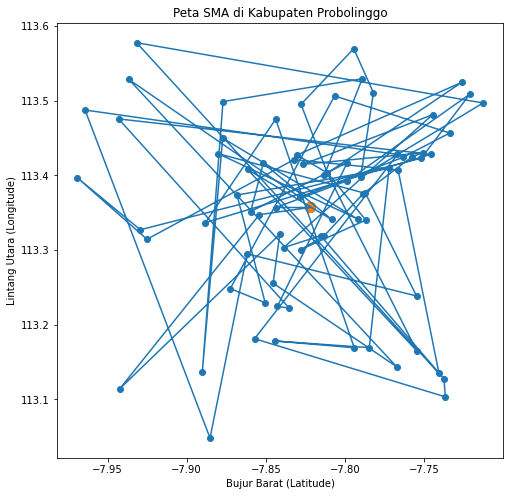
\includegraphics[width=0.5\textwidth]{Gambar/hasil_mtsp/1}
\caption{Perjalanan tanpa pembagian klaster}
\label{fig:hasil_mtsp1}
\end{figure}

\subsection{Pembagian 2 klaster}

Pada tahap ini urutan perjalanan dibagi menjadi 2 klaster yaitu klaster A dan B, menghasilkan urutan sebagai berikut.

\begin{enumerate}
\item Urutan perjalanan pada klaster A:

$
33 \rightarrow 17 \rightarrow 47 \rightarrow 32 \rightarrow 55 \rightarrow 36 \rightarrow 10 \rightarrow 37 \rightarrow 56 \rightarrow 11 \rightarrow 30 \rightarrow 27 \rightarrow 59 \rightarrow 60 \rightarrow 64 \rightarrow 21 \rightarrow 9 \rightarrow 39 \rightarrow 29 \rightarrow 24 \rightarrow 63 \rightarrow 72 \rightarrow 13 \rightarrow 6 \rightarrow 38 \rightarrow 52
$

\item Urutan perjalanan pada klaster B:

\noindent $
43 \rightarrow 35 \rightarrow 7 \rightarrow 2 \rightarrow 44 \rightarrow 25 \rightarrow 70 \rightarrow 61 \rightarrow 66 \rightarrow 45 \rightarrow 68 \rightarrow 65 \rightarrow 50 \rightarrow 22 \rightarrow 46 \rightarrow 49 \rightarrow 14 \rightarrow 5 \rightarrow 16 \rightarrow 74 \rightarrow 42 \rightarrow 8 \rightarrow 48 \rightarrow 31 \rightarrow 26 \rightarrow 18 \rightarrow 54 \rightarrow 40 \rightarrow 58 \rightarrow 67 \rightarrow 15 \rightarrow 12 \rightarrow 57 \rightarrow 20 \rightarrow 34 \rightarrow 69 \rightarrow 75 \rightarrow 41 \rightarrow 23 \rightarrow 51 \rightarrow 19 \rightarrow 28 \rightarrow 1 \rightarrow 62 \rightarrow 4 \rightarrow 53 \rightarrow 3 \rightarrow 71 \rightarrow 73
$
\end{enumerate}

Dapat dilihat pada Gambar \ref{fig:hasil_mtsp2} perjalanan menuju seluruh SMA di Kabupaten Probolinggo dengan dibagi menjadi 2 klaster. Terlihat pada urutan tersebut menghasilkan jarak total seperti pada Tabel \ref{tab:totaljarak} yaitu $7,45$ satuan.

\begin{figure}[H]
\centering
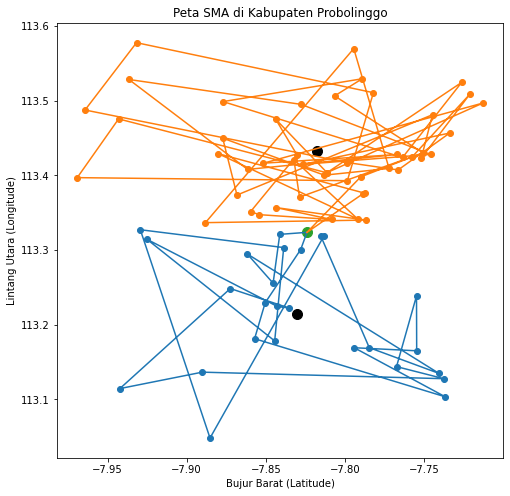
\includegraphics[width=0.5\textwidth]{Gambar/hasil_mtsp/2}
\caption{Perjalanan dibagi 2 klaster}
\label{fig:hasil_mtsp2}
\end{figure}

\subsection{Pembagian 3 klaster}

Pada tahap ini urutan perjalanan dibagi menjadi 3 klaster yaitu klaster A, B, dan C, menghasilkan urutan perjalanan sebagai berikut.

\begin{enumerate}
\item Urutan perjalanan pada klaster A:

$
38 \rightarrow 60 \rightarrow 56 \rightarrow 32 \rightarrow 13 \rightarrow 21 \rightarrow 72 \rightarrow 47 \rightarrow 59 \rightarrow 36 \rightarrow 37 \rightarrow 55 \rightarrow 27 \rightarrow 17 \rightarrow 29 \rightarrow 30 \rightarrow 11 \rightarrow 10
$ 

\item Urutan perjalanan pada klaster B:

$
2 \rightarrow 66 \rightarrow 14 \rightarrow 74 \rightarrow 26 \rightarrow 42 \rightarrow 54 \rightarrow 22 \rightarrow 51 \rightarrow 50 \rightarrow 34 \rightarrow 70 \rightarrow 7 \rightarrow 28 \rightarrow 8 \rightarrow 44 \rightarrow 41
$

\item Urutan perjalanan pada klaster C:

$
69 \rightarrow 68 \rightarrow 40 \rightarrow 73 \rightarrow 25 \rightarrow 5 \rightarrow 1 \rightarrow 35 \rightarrow 65 \rightarrow 3 \rightarrow 24 \rightarrow 16 \rightarrow 19 \rightarrow 71 \rightarrow 61 \rightarrow 58 \rightarrow 53 \rightarrow 23 \rightarrow 49 \rightarrow 67 \rightarrow 64 \rightarrow 33 \rightarrow 4 \rightarrow 18 \rightarrow 39 \rightarrow 48 \rightarrow 20 \rightarrow 75 \rightarrow 63 \rightarrow 15 \rightarrow 31 \rightarrow 43 \rightarrow 57 \rightarrow 9 \rightarrow 6 \rightarrow 12 \rightarrow 46 \rightarrow 45 \rightarrow 52 \rightarrow 62
$
\end{enumerate}

Dapat dilihat pada Gambar \ref{fig:hasil_mtsp3} perjalanan menuju seluruh SMA di Kabupaten Probolinggo dibagi menjadi 3 klaster. Terlihat pada urutan tersebut menghasilkan jarak total pada Tabel \ref{tab:totaljarak} yaitu $6,44$ satuan.

\begin{figure}[H]
\centering
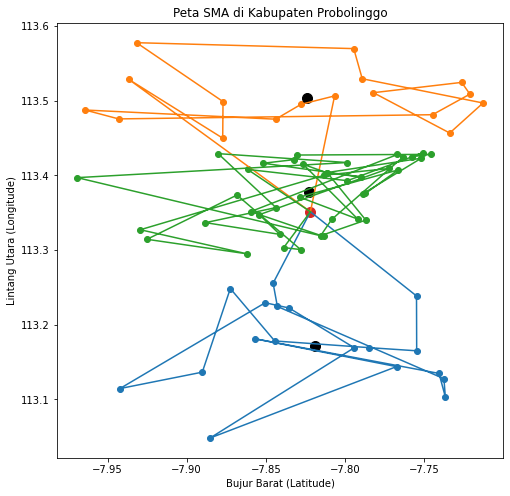
\includegraphics[width=0.5\textwidth]{Gambar/hasil_mtsp/3}
\caption{Perjalanan dibagi 3 klaster}
\label{fig:hasil_mtsp3}
\end{figure}

\subsection{Pembagian 4 klaster}

Pada tahap ini urutan perjalanan dibagi menjadi 4 klaster yaitu klaster A, B, C, dan D, menghasilkan urutan perjalanan sebagai berikut.

\begin{enumerate}

\item Urutan perjalanan pada klaster A:

$60\rightarrow36\rightarrow72\rightarrow21\rightarrow11\rightarrow13\rightarrow55\rightarrow56\rightarrow32\rightarrow27\rightarrow38\rightarrow10\rightarrow59\rightarrow30\rightarrow37\rightarrow29\rightarrow47\rightarrow17$

\item Urutan perjalanan pada klaster B:

$54\rightarrow34\rightarrow2\rightarrow42\rightarrow22\rightarrow50\rightarrow44\rightarrow7\rightarrow28\rightarrow51\rightarrow66\rightarrow8\rightarrow70$

\item Urutan perjalanan pada klaster C:

$18\rightarrow61\rightarrow4\rightarrow40\rightarrow71\rightarrow53\rightarrow57\rightarrow16\rightarrow1\rightarrow46\rightarrow19\rightarrow14\rightarrow75\rightarrow49\rightarrow5\rightarrow68\rightarrow69\rightarrow73\rightarrow25\rightarrow43\rightarrow48\rightarrow35\rightarrow15$

\item Urutan perjalanan pada klaster D:

$62\rightarrow24\rightarrow6\rightarrow65\rightarrow67\rightarrow20\rightarrow23\rightarrow12\rightarrow33\rightarrow9\rightarrow63\rightarrow45\rightarrow41\rightarrow74\rightarrow31\rightarrow39\rightarrow64\rightarrow52\rightarrow58\rightarrow3\rightarrow26$

\end{enumerate}

Dapat dilihat pada Gambar \ref{fig:hasil_mtsp4} perjalanan menuju seluru SMA di Kabupaten Probolinggo dibagi menjadi 4 klaster. Terlihat pada urutan tersebut menghasilkan jarak total pada Tabel \ref{tab:totaljarak} yaitu $5,45$ satuan

\begin{figure}[H]
\centering
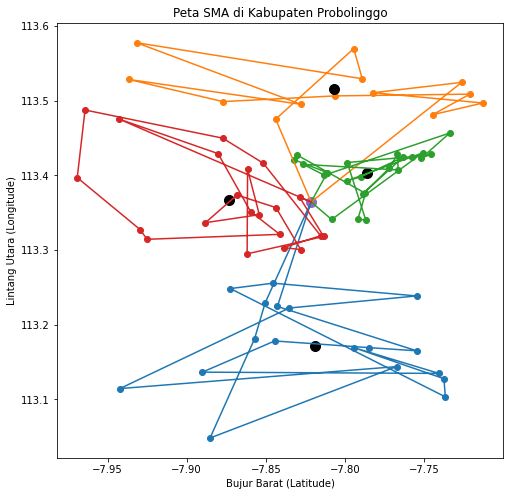
\includegraphics[width=0.5\textwidth]{Gambar/hasil_mtsp/4}
\caption{Perjalanan dibagi 4 klaster}
\label{fig:hasil_mtsp4}
\end{figure}

\subsection{Pembagian 5 klaster}

Pada tahap ini urutan perjalanan dibagi menjadi 5 klaster yaitu klaster A, B, C, D, dan E, menghasilkan urutan perjalanan sebagai berikut.

\begin{enumerate}

\item Urutan perjalanan pada klaster A:

$10\rightarrow36\rightarrow13\rightarrow56\rightarrow60\rightarrow37\rightarrow21\rightarrow55\rightarrow59\rightarrow72\rightarrow32\rightarrow29\rightarrow47\rightarrow17\rightarrow11\rightarrow30$

\item Urutan perjalanan pada klaster B:

$8\rightarrow34\rightarrow7\rightarrow22\rightarrow28\rightarrow66\rightarrow51\rightarrow14\rightarrow70\rightarrow2$

\item Urutan perjalanan pada klaster C:

$62\rightarrow71\rightarrow43\rightarrow35\rightarrow16\rightarrow61\rightarrow5\rightarrow18\rightarrow75\rightarrow4\rightarrow69\rightarrow1\rightarrow45\rightarrow73\rightarrow49\rightarrow68\rightarrow19\rightarrow25\rightarrow46\rightarrow48\rightarrow65\rightarrow40\rightarrow53\rightarrow57$

\item Urutan perjalanan pada klaster D:

$52\rightarrow6\rightarrow33\rightarrow20\rightarrow23\rightarrow15\rightarrow24\rightarrow64\rightarrow39\rightarrow27\rightarrow38\rightarrow63\rightarrow67\rightarrow58\rightarrow9\rightarrow12$

\item Urutan perjalanan pada klaster E:

$41\rightarrow42\rightarrow50\rightarrow74\rightarrow44\rightarrow26\rightarrow31\rightarrow54\rightarrow3$

\end{enumerate}

Dapat dilihat pada Gambar \ref{fig:hasil_mtsp5} perjalanan menuju seluru SMA di Kabupaten Probolinggo dibagi menjadi 5 klaster. Terlihat pada urutan tersebut menghasilkan jarak total pada Tabel \ref{tab:totaljarak} yaitu $5,45$ satuan

\begin{figure}[H]
\centering
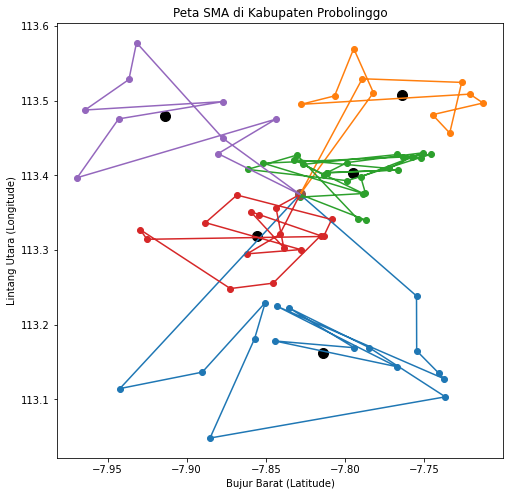
\includegraphics[width=0.5\textwidth]{Gambar/hasil_mtsp/5}
\caption{Perjalanan dibagi 5 klaster}
\label{fig:hasil_mtsp5}
\end{figure}

\subsection{Pembagian 6 klaster}

Pada tahap ini urutan perjalanan dibagi menjadi 6 klaster yaitu klaster A, B, C, D, E, dan F, menghasilkan urutan perjalanan sebagai berikut.

\begin{enumerate}

\item Urutan perjalanan pada klaster A:

$30\rightarrow11\rightarrow29\rightarrow37\rightarrow36\rightarrow13\rightarrow32\rightarrow56\rightarrow55\rightarrow72$

\item Urutan perjalanan pada klaster B:

$14\rightarrow70\rightarrow28\rightarrow34\rightarrow2\rightarrow66\rightarrow22\rightarrow51\rightarrow8\rightarrow7$

\item Urutan perjalanan pada klaster C:

$69\rightarrow1\rightarrow19\rightarrow75\rightarrow71\rightarrow68\rightarrow48\rightarrow65\rightarrow25\rightarrow16\rightarrow45\rightarrow4\rightarrow18\rightarrow40\rightarrow43\rightarrow73\rightarrow35\rightarrow46\rightarrow5\rightarrow49\rightarrow61$

\item Urutan perjalanan pada klaster D:

$58\rightarrow53\rightarrow57\rightarrow15\rightarrow39\rightarrow64\rightarrow52\rightarrow20\rightarrow23\rightarrow67\rightarrow24\rightarrow62\rightarrow63\rightarrow12\rightarrow6\rightarrow9\rightarrow33$

\item Urutan perjalanan pada klaster E:

$54\rightarrow50\rightarrow42\rightarrow31\rightarrow74\rightarrow26\rightarrow44\rightarrow41\rightarrow3$

\item Urutan perjalanan pada klaster F:

$10\rightarrow21\rightarrow47\rightarrow17\rightarrow60\rightarrow59\rightarrow38\rightarrow27$

\end{enumerate}

Dapat dilihat pada Gambar \ref{fig:hasil_mtsp6} perjalanan menuju seluru SMA di Kabupaten Probolinggo dibagi menjadi 6 klaster. Terlihat pada urutan tersebut menghasilkan jarak total pada Tabel \ref{tab:totaljarak} yaitu $4,89$ satuan

\begin{figure}[H]
\centering
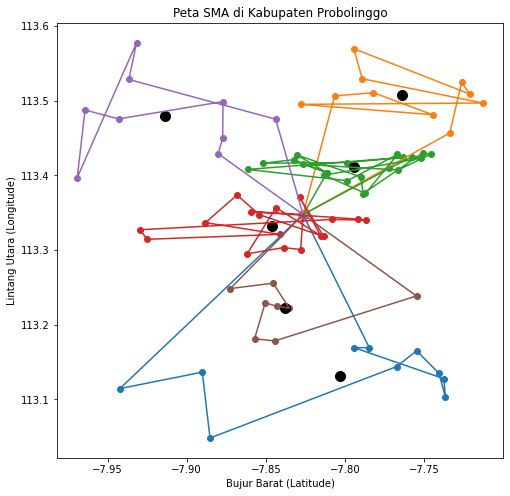
\includegraphics[width=0.5\textwidth]{Gambar/hasil_mtsp/6}
\caption{Perjalanan dibagi 6 klaster}
\label{fig:hasil_mtsp6}
\end{figure}

\subsection{Pembagian 7 klaster}

Pada tahap ini urutan perjalanan dibagi menjadi 7 klaster yaitu klaster A, B, C, D, E, F, dan G, menghasilkan urutan perjalanan sebagai berikut.

\begin{enumerate}

\item Urutan perjalanan pada klaster A:

$13\rightarrow56\rightarrow36\rightarrow37\rightarrow11\rightarrow30\rightarrow21\rightarrow47\rightarrow32\rightarrow29\rightarrow55\rightarrow72$

\item Urutan perjalanan pada klaster B:

$22\rightarrow7\rightarrow70\rightarrow28\rightarrow66\rightarrow34\rightarrow2\rightarrow8\rightarrow51$

\item Urutan perjalanan pada klaster C:

$71\rightarrow43\rightarrow5\rightarrow25\rightarrow68\rightarrow48\rightarrow16\rightarrow69\rightarrow57\rightarrow53\rightarrow73\rightarrow35\rightarrow14\rightarrow46\rightarrow1\rightarrow19$

\item Urutan perjalanan pada klaster D:

$15\rightarrow52\rightarrow31\rightarrow64\rightarrow12\rightarrow23\rightarrow20\rightarrow58\rightarrow67\rightarrow39$

\item Urutan perjalanan pada klaster E:

$44\rightarrow50\rightarrow42\rightarrow74\rightarrow26$

\item Urutan perjalanan pada klaster F:

$63\rightarrow6\rightarrow38\rightarrow17\rightarrow24\rightarrow33\rightarrow27\rightarrow60\rightarrow59\rightarrow10\rightarrow9$

\item Urutan perjalanan pada klaster G:

$4\rightarrow40\rightarrow45\rightarrow49\rightarrow75\rightarrow41\rightarrow54\rightarrow3\rightarrow65\rightarrow61\rightarrow18\rightarrow62$

\end{enumerate}

Dapat dilihat pada Gambar \ref{fig:hasil_mtsp7} perjalanan menuju seluru SMA di Kabupaten Probolinggo dibagi menjadi 7 klaster. Terlihat pada urutan tersebut menghaslilkan jarak total pada Tabel \ref{tab:totaljarak} yaitu $4,85$ satuan.

\begin{figure}[H]
\centering
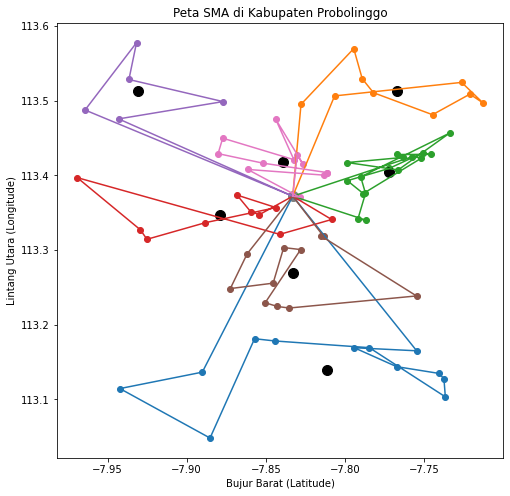
\includegraphics[width=0.5\textwidth]{Gambar/hasil_mtsp/7}
\caption{Perjalanan dibagi 7 klaster}
\label{fig:hasil_mtsp7}
\end{figure}

\subsection{Pembagian 8 klaster}

Pada tahap ini urutan perjalanan dibagi menjadi 8 klaster yaitu klaster A, B, C, D, E, F, G, dan H, menghasilkan urutan perjalanan sebagai berikut.

\begin{enumerate}
\item Urutan perjalanan pada klaster A:

$11\rightarrow21\rightarrow30\rightarrow29\rightarrow37\rightarrow56\rightarrow13\rightarrow55\rightarrow36\rightarrow32\rightarrow72\rightarrow47$

\item Urutan perjalanan pada klaster B:

$22\rightarrow7\rightarrow70\rightarrow28\rightarrow66\rightarrow34\rightarrow2\rightarrow8\rightarrow51$

\item Urutan perjalanan pada klaster C:

$43\rightarrow25\rightarrow46\rightarrow35\rightarrow19\rightarrow5\rightarrow69\rightarrow16\rightarrow68\rightarrow14\rightarrow1\rightarrow48$

\item Urutan perjalanan pada klaster D:

$23\rightarrow31\rightarrow20\rightarrow39\rightarrow64$

\item Urutan perjalanan pada klaster E:

$44\rightarrow42\rightarrow26\rightarrow50\rightarrow74$

\item Urutan perjalanan pada klaster F:

$59\rightarrow60\rightarrow27\rightarrow6\rightarrow38\rightarrow10\rightarrow33\rightarrow9\rightarrow17$

\item Urutan perjalanan pada klaster G:

$4\rightarrow3\rightarrow54\rightarrow65\rightarrow40\rightarrow41\rightarrow45\rightarrow18\rightarrow75\rightarrow61\rightarrow49$

\item Urutan perjalanan pada klaster H:

$52\rightarrow67\rightarrow58\rightarrow62\rightarrow15\rightarrow57\rightarrow53\rightarrow24\rightarrow63\rightarrow73\rightarrow71\rightarrow12$
\end{enumerate}

Dapat dilihat pada Gambar \ref{fig:hasil_mtsp8} perjalanan menuju seluru SMA di Kabupaten Probolinggo dibagi menjadi 8 klaster. Terlihat pada urutan tersebut menghaslilkan jarak total pada Tabel \ref{tab:totaljarak} yaitu $4,76$ satuan. Nilai jarak total pada pembagian klaster ini merupakan jarak total yang paling rendah diantara yang lain.

\begin{figure}[H]
\centering
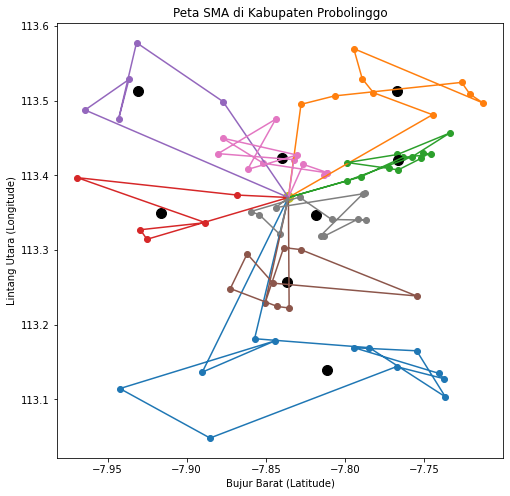
\includegraphics[width=0.5\textwidth]{Gambar/hasil_mtsp/8}
\caption{Perjalanan dibagi 8 klaster}
\label{fig:hasil_mtsp8}
\end{figure}

\subsection{Pembagian 9 klaster}

Pada tahap ini urutan perjalanan dibagi menjadi 9 klaster yaitu klaster A, B, C, D, E, F, G, H, dan I, menghasilkan urutan perjalanan sebagai berikut.

\begin{enumerate}
\item Urutan perjalanan pada klaster A:

$17\rightarrow60\rightarrow21\rightarrow47\rightarrow59\rightarrow10$

\item Urutan perjalanan pada klaster B:

$2\rightarrow22\rightarrow7\rightarrow51\rightarrow8\rightarrow66\rightarrow28\rightarrow34\rightarrow70$

\item Urutan perjalanan pada klaster C:

$69\rightarrow1\rightarrow68\rightarrow19\rightarrow35\rightarrow14\rightarrow5\rightarrow46\rightarrow25\rightarrow43\rightarrow16$

\item Urutan perjalanan pada klaster D:

$67\rightarrow23\rightarrow58\rightarrow31\rightarrow39\rightarrow20\rightarrow64$

\item Urutan perjalanan pada klaster E:

$74\rightarrow42\rightarrow50\rightarrow26\rightarrow44$

\item Urutan perjalanan pada klaster F:

$52\rightarrow6\rightarrow27\rightarrow38\rightarrow33\rightarrow9$

\item Urutan perjalanan pada klaster G:

$3\rightarrow45\rightarrow65\rightarrow54\rightarrow41\rightarrow40\rightarrow61\rightarrow49\rightarrow75\rightarrow4\rightarrow18$

\item Urutan perjalanan pada klaster H:

$62\rightarrow12\rightarrow63\rightarrow57\rightarrow53\rightarrow24\rightarrow48\rightarrow73\rightarrow71\rightarrow15$

\item Urutan perjalanan pada klaster I:

$13\rightarrow32\rightarrow37\rightarrow30\rightarrow29\rightarrow56\rightarrow11\rightarrow72\rightarrow55\rightarrow36$

\end{enumerate}

Dapat dilihat pada Gambar \ref{fig:hasil_mtsp9} perjalanan menuju seluru SMA di Kabupaten Probolinggo dibagi menjadi 9 klaster. Terlihat pada urutan tersebut menghaslilkan jarak total pada Tabel \ref{tab:totaljarak} yaitu $5,08$ satuan.

\begin{figure}[H]
\centering
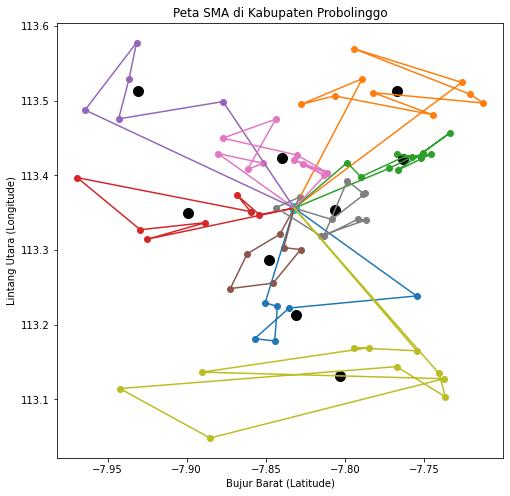
\includegraphics[width=0.5\textwidth]{Gambar/hasil_mtsp/9}
\caption{Perjalanan dibagi 9 klaster}
\label{fig:hasil_mtsp9}
\end{figure}

\subsection{Pembagian 10 klaster}

Pada tahap ini urutan perjalanan dibagi menjadi 10 klaster yaitu klaster A, B, C, D, E, F, G, H, I, dan J, menghasilkan urutan perjalanan sebagai berikut.

\begin{enumerate}
\item Urutan perjalanan pada klaster A:

$59\rightarrow21\rightarrow17\rightarrow60\rightarrow47\rightarrow10$

\item Urutan perjalanan pada klaster B:

$2\rightarrow22\rightarrow7\rightarrow51\rightarrow8\rightarrow66\rightarrow28\rightarrow34\rightarrow70$

\item Urutan perjalanan pada klaster C:

$69\rightarrow1\rightarrow68\rightarrow19\rightarrow35\rightarrow14\rightarrow5\rightarrow46\rightarrow25\rightarrow43\rightarrow16$

\item Urutan perjalanan pada klaster D:

$23\rightarrow52\rightarrow39\rightarrow64\rightarrow58\rightarrow20\rightarrow67\rightarrow12$

\item Urutan perjalanan pada klaster E:

$26\rightarrow74\rightarrow31$

\item Urutan perjalanan pada klaster F:

$6\rightarrow27\rightarrow38\rightarrow33\rightarrow9$

\item Urutan perjalanan pada klaster G:

$65\rightarrow45\rightarrow41\rightarrow4\rightarrow3\rightarrow54\rightarrow40\rightarrow49\rightarrow75\rightarrow18\rightarrow61$

\item Urutan perjalanan pada klaster H:

$62\rightarrow48\rightarrow53\rightarrow73\rightarrow71\rightarrow24\rightarrow57\rightarrow15\rightarrow63$

\item Urutan perjalanan pada klaster I:

$11\rightarrow30\rightarrow29\rightarrow13\rightarrow36\rightarrow55\rightarrow32\rightarrow56\rightarrow37\rightarrow72$

\item Urutan perjalanan pada klaster J:

$44\rightarrow50\rightarrow42$

\end{enumerate}

Dapat dilihat pada Gambar \ref{fig:hasil_mtsp10} perjalanan menuju seluru SMA di Kabupaten Probolinggo dibagi menjadi 10 klaster. Terlihat pada urutan tersebut menghaslilkan jarak total pada Tabel \ref{tab:totaljarak} yaitu $5,02$ satuan.

\begin{figure}[H]
\centering
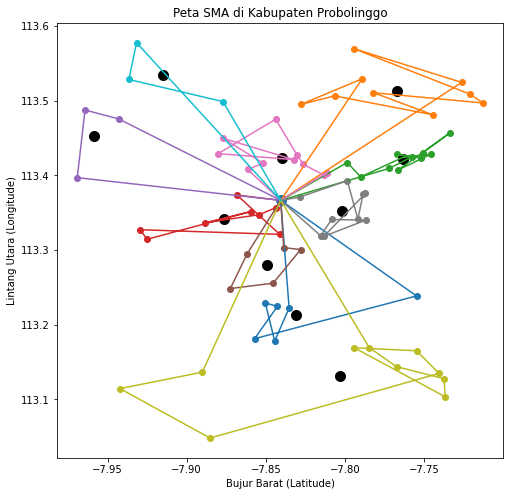
\includegraphics[width=0.5\textwidth]{Gambar/hasil_mtsp/10}
\caption{Perjalanan dibagi 10 klaster}
\label{fig:hasil_mtsp10}
\end{figure}

\begin{table}[H]
\centering
\footnotesize
\begin{tabular}{ccccc}
\rowcolor[HTML]{4472C4} 
\cellcolor[HTML]{4472C4}{\color[HTML]{FFFFFF} } &
  \cellcolor[HTML]{4472C4}{\color[HTML]{FFFFFF} } &
  \cellcolor[HTML]{4472C4}{\color[HTML]{FFFFFF} } &
  \multicolumn{2}{c}{\cellcolor[HTML]{4472C4}{\color[HTML]{FFFFFF} \textbf{Titik Kumpul}}} \\
\rowcolor[HTML]{4472C4} 
\multirow{-2}{*}{\cellcolor[HTML]{4472C4}{\color[HTML]{FFFFFF} \textbf{Banyak Klaster}}} &
  \multirow{-2}{*}{\cellcolor[HTML]{4472C4}{\color[HTML]{FFFFFF} \textbf{Total Jarak}}} &
  \multirow{-2}{*}{\cellcolor[HTML]{4472C4}{\color[HTML]{FFFFFF} \textbf{Peringkat}}} &
  \cellcolor[HTML]{4472C4}{\color[HTML]{FFFFFF} \textbf{Latitude (X)}} &
  \cellcolor[HTML]{4472C4}{\color[HTML]{FFFFFF} \textbf{Longitude (Y)}} \\
1  & 10,0503  & 10 & -7,8221841 & 113,3570412 \\
\rowcolor[HTML]{D9E1F2} 
2  & 6,858777 & 9  & -7,8241236 & 113,3236903 \\
3  & 5,599878 & 8  & -7,8219762 & 113,3512877 \\
\rowcolor[HTML]{D9E1F2} 
4  & 5,010994 & 7  & -7,8215022 & 113,3644199 \\
5  & 4,805015 & 6  & -7,828521  & 113,3744846 \\
\rowcolor[HTML]{D9E1F2} 
6  & 4,43132  & 3  & -7,8265701 & 113,3475373 \\
7  & 4,353295 & 1  & -7,8331118 & 113,3721289 \\
\rowcolor[HTML]{D9E1F2} 
8  & 4,398984 & 2  & -7,8358502 & 113,3704048 \\
9  & 4,48243  & 4  & -7,8321462 & 113,356253  \\
\rowcolor[HTML]{D9E1F2} 
10 & 4,780413 & 5  & -7,8406976 & 113,3665328
\end{tabular}
\caption{Total jarak dengan jumlah pembagian klaster yang berbeda}
\label{tab:totaljarak}
\end{table}